\documentclass{article}
\usepackage{../../Self_Style}

\title{Phys 20AL Week 4: Mass and Spring}
\author{Zih-Yu Hsieh}
\date{\today}

\begin{document}
\maketitle

\section{Aim for Experiment}
The experiment is to measure the spring constant of a spring (which is a simple harmonic oscillator). In addition, it'll also be focusing on the static relation between the mass and the spring stretch of a spring, together with how variation of mass and maximum amplitude would affect the time period of a spring's dynamic motion.

\section{Experimental Setup}
Here there are three different sets of experiments, where two of them uses one setup, while the last one uses the other.

\subsection{Experiments Recording data Manually}
For this setup, there are two experiments involved: Collecting data of the spring's stretch under static scenario, and collecting data of the object's period under dynamic scenario.

The equipments include: Stand, two clamps, spring (that can endure long enough stretch without explicit deformation, typically a stretch of near $1$ m), meter stick, a hook of $50$ g, timer, mass scale, and masses of one $50$ g, two $100$ g, and one $200$ g.

The following is the steps for setup:
\begin{itemize}
    \item[1.] Setup the stand at the edge of the table.
    \item[2.] Fix one of the clamp on the top of the stand, and clamp one end of the spring onto it.
    \item[3.] Fix the other clamp near the middle of the stand, and clamp the meter stick vertically onto it.
\end{itemize}
\begin{figure}[h!]
    \centering
    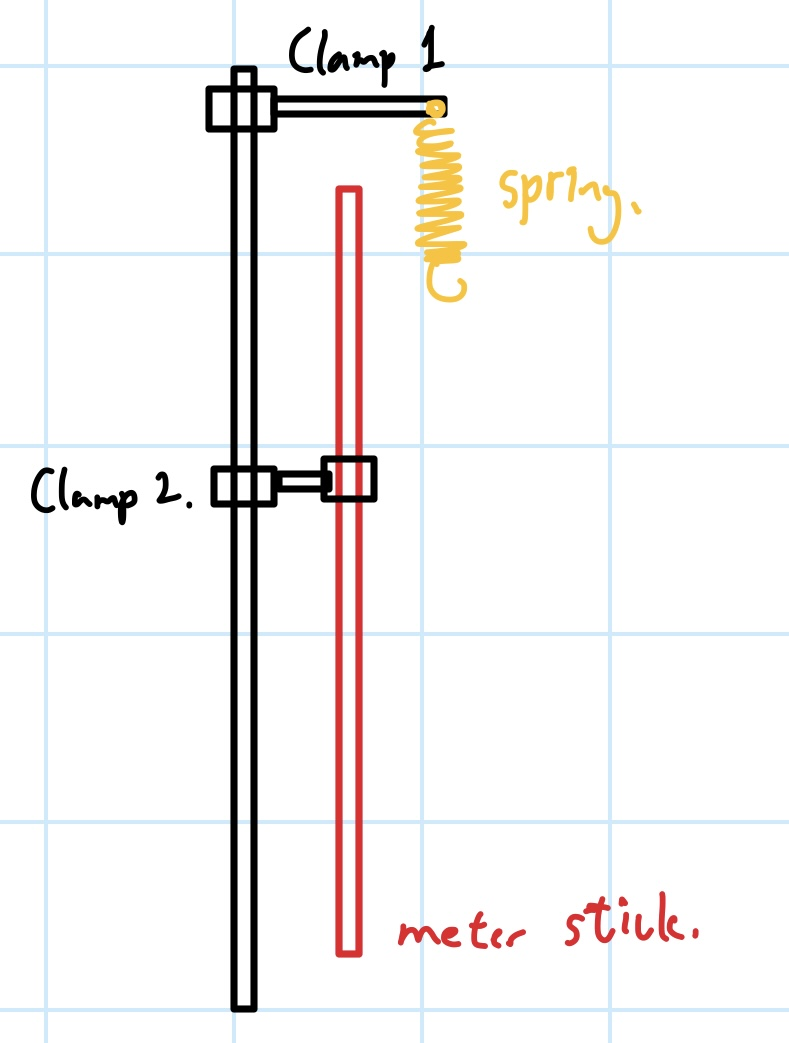
\includegraphics[width=40mm]{setup_sketch_manual.jpg}
    \caption{Sketch of the Setup with Manual Data Recording}
\end{figure}

\subsection{Experiment Recording data with Detector}
For this setup, there is only one experiment, which is using the electronic detector to record the dynamic motion of the simple harmonic oscillator.

The equipments are nearly the same as in \textbf{Section 2.1}, except now it requires one more clamp, an electronic detector, and a computer.

The setup steps mostly follow from the one in \textbf{Section 2.1}, just additionally one needs to use the extra clamp to fix the detector on the stand, and plugin the detector to the computer for data recording.
\begin{figure}[h!]
    \centering
    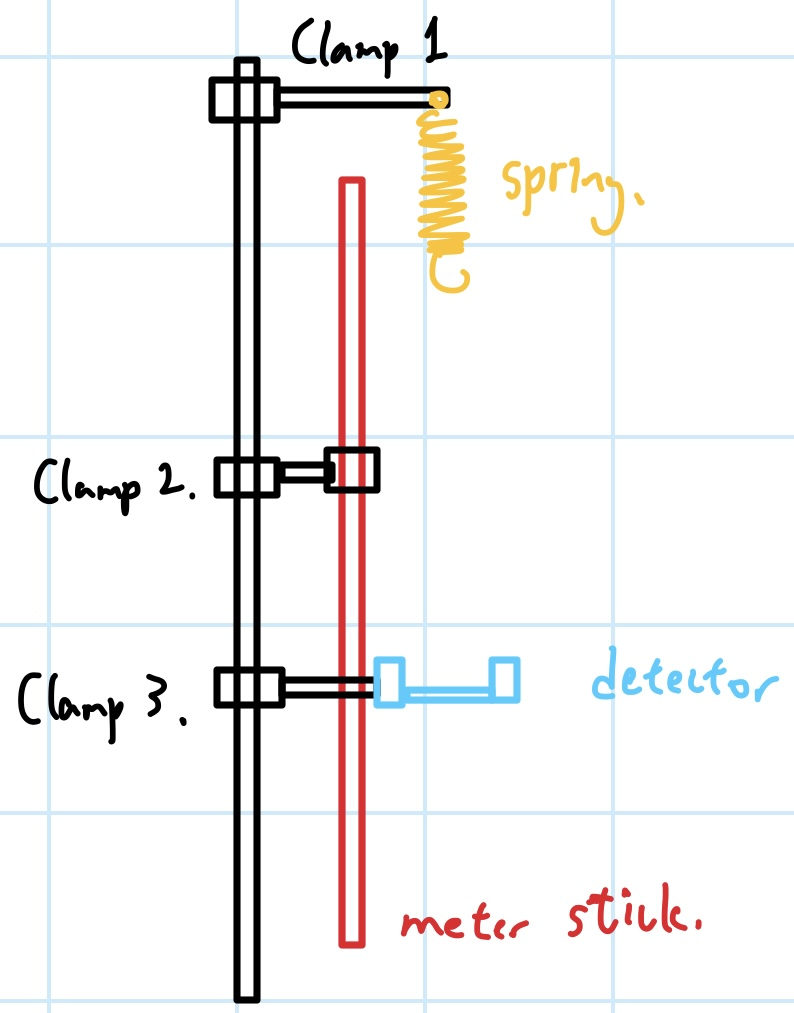
\includegraphics[width=40mm]{setup_sketch_detector.jpg}
    \caption{Sketch of the Setup with Manual Data Recording}
\end{figure}


\section{Measurement \& Method of Measure}
In all the experiments, for any pairs of manipulated variables, we'll do a total of $3$ trials each.
\subsection{Static Approach}
For the static approach, the aim is to measure when varying the mass (which corresponds to different gravitational force applied on the spring), how far the spring has stretched from original weightless scenario after the spring system reaches static equilibrium when the mass is added.

Here, the mass will be measured using a mass scale (unit: kg), and the stretch of the spring will be measured through the meter stick (unit: m). Which, the masses being tested are given by $n \cdot 50$ g (where integer $n$ satisfies $1\leq n\leq 10$). In terms of kg, it's given by $n \cdot 0.05$ kg, for every integer $n$ satisfying $1\leq n\leq 10$.

\subsection{Dynamic Approach}
For the dynamic approach, the aim is to measure the time period for the spring (i.e. a simple harmonic oscillator) to complete a cycle, and to observe how varying the mass and maximum amplitude of the spring system would affect this time period.

The mass measurement would again be done by a mass scale (unit: kg), and the maximum amplitude of the oscillation will be measured through the meter stick (unit: m). The time period measurement then differ depending on the experiment:
\begin{itemize}
    \item For the experiment recording data manually, we'll use a timer to measure the time period (unit: s).
    \item For the experiment recording data with detector, the electronic detector serve as an automated timer for measurement.
\end{itemize}
In both cases, we'll let the spring oscillates in total of $5$ times, and record the total tie elapsed for the five cycles.

\hfil

For both experiments, the proposed maximum amplitudes are $2,4,6$ cm respectively (or $0.02,0.04,0.06$ m).

For the mass that will be used, it differs by the experiment:
\begin{itemize}
    \item For the experiment measuring time manually, the mass will be $100,200,300$ g respectively (or $0.1,0.2,0.3$ kg respectively).
    \item For the experiment measuring time with detector, the mass will be $100,150,200$ g respectively (or $0.1,0.15,0.2$ kg).
\end{itemize}

\section{Experimental Procedure}
\subsection{Static Approach}
We'll follow the procedure below:
\begin{itemize}
    \item[1.] Measure the initial static equilibrium point of the spring's free end using the meter stick (where meter stick should be fixed at the same height across the whole experiment).
    \item[2.] Fix a mass that's going to be tested, put the mass on the hook, and hang the hook on the free end of the spring.
    \item[3.] Wait till the spring system be at static equilibrium, then measure the new static equilibrium point of the spring's free end.
    \item[4.] Record the difference of this new position away from the initial position recorded in Step 1. 
    \item[5.] Repeat Step 2 to 4 in total of three trials.
    \item[6.] Change the mass to other ones awaited to be tested, and repeat Step 2 to 5 for each mass.  
\end{itemize}
\textbf{Rmk:} any mass with the form $n\cdot 50$ g (where integer $1\leq n\leq 10$) can be formed using two $50$ g, two $100$ g, and one $200$ g, so the provided masses can complete the experiment.

\subsection{Dynamic Approach}
\subsubsection{Experiment without Detector}
We'll follow the procedure below:
\begin{itemize}
    \item[1.] Fix a mass that is being used, put the mass onto the hook, and hang it onto the spring until it reaches sattic equilibrium.
    \item[2.] Fix a maximum amplitude that is being used (say $l$), pull the spring down until it is distance $l$ away from the equilibrium point.
    \item[3.] Release the spring, and start the timer simulteneously. Wait until the spring oscillates total of $5$ cycles and record the time it takes to complete it.
    \item[4.] Repeat Step 2 to 3 for a total of three trials. 
    \item[5.] Change the maximum amplitude to other values await to be tested, and repeat Step 2 to 4 for each desired maximum amplitude.
    \item[6.] Change the mass to other values await to be tested, and repeat Step 2 to 5 for each mass.   
\end{itemize}

\subsubsection{Experiment with Detector}
For the case with detector, it merely follows the procedure used in \textbf{Section 4.2.2}, except the timer's measurement is swapped using the detector.

As a remark, needs to make sure when starting the measurement, the detector is right on the equilibrium point (so if the mass varies, causing the equilibrium to change, need to adjust the height of the detector accordingly through fixing the clamp at corresponding height).

\section{Experimental Data}
\subsection{Static Approach}
\begin{figure}[h!]
    \centering
    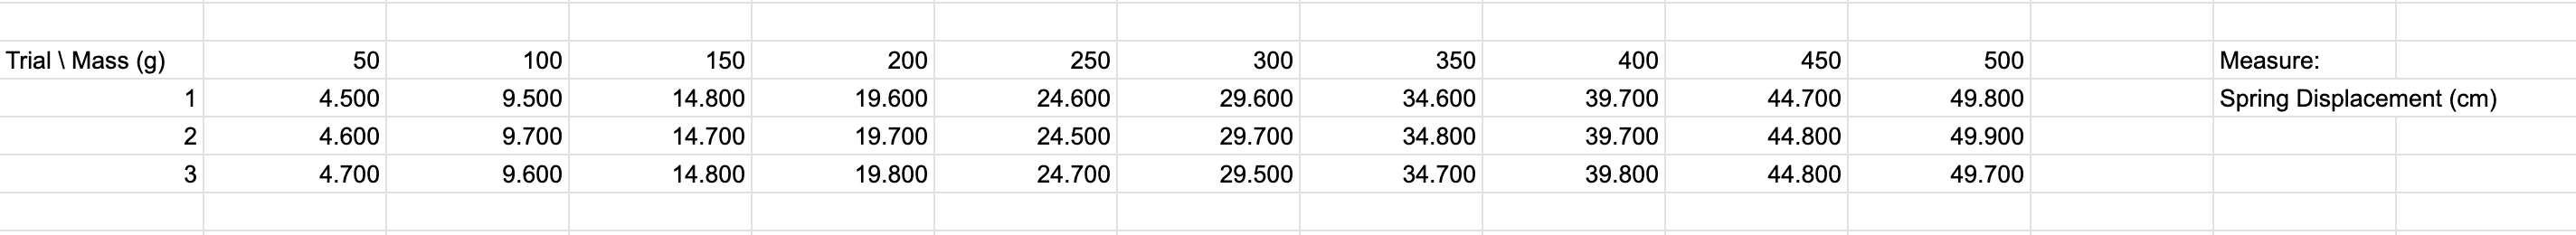
\includegraphics[width=170mm]{static_dataa.png}
\end{figure}
\begin{figure}[h!]
    \centering
    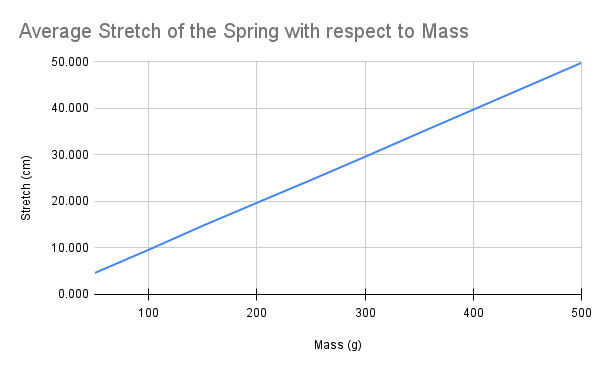
\includegraphics[width=100mm]{Average Stretch of the Spring with respect to Mass.png}
\end{figure}

\newpage

\subsection{Dynamic Approach - Manual Recording}
\begin{figure}[ht!]
    \centering
    %top row
    \begin{subfigure}{0.8\textwidth}
        \centering
        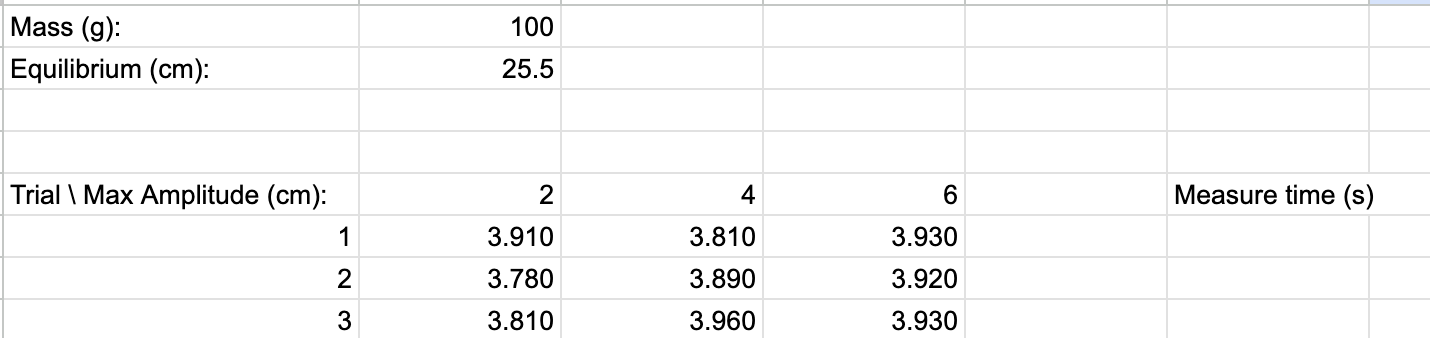
\includegraphics[width=\linewidth]{dynamic_1.png}
        \label{fig:graph_m1}
    \end{subfigure}
    
    \vspace{1em}

    \begin{subfigure}{0.8\textwidth}
        \centering
        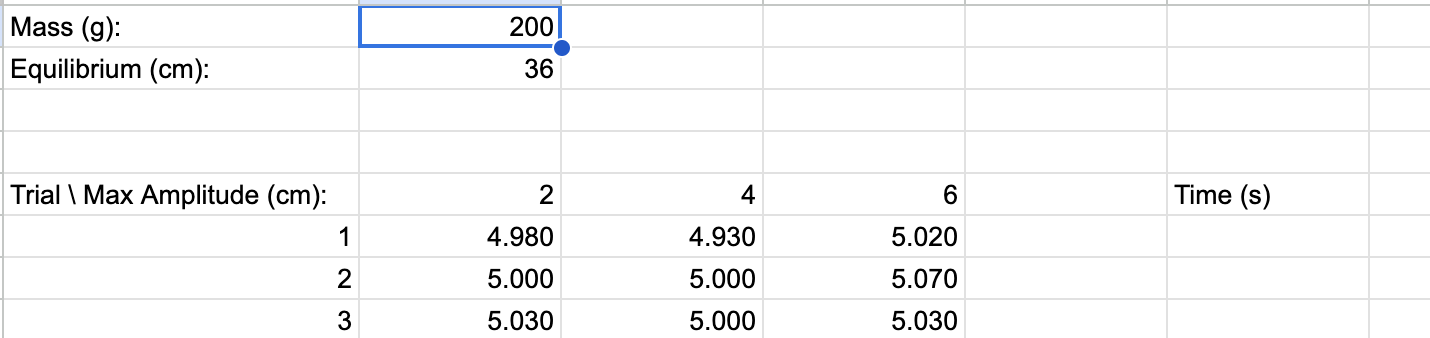
\includegraphics[width=\linewidth]{dynamic_2.png}
        \label{fig:graph_m2}
    \end{subfigure}
    
    \vspace{1em}

    \begin{subfigure}{0.8\textwidth}
        \centering
        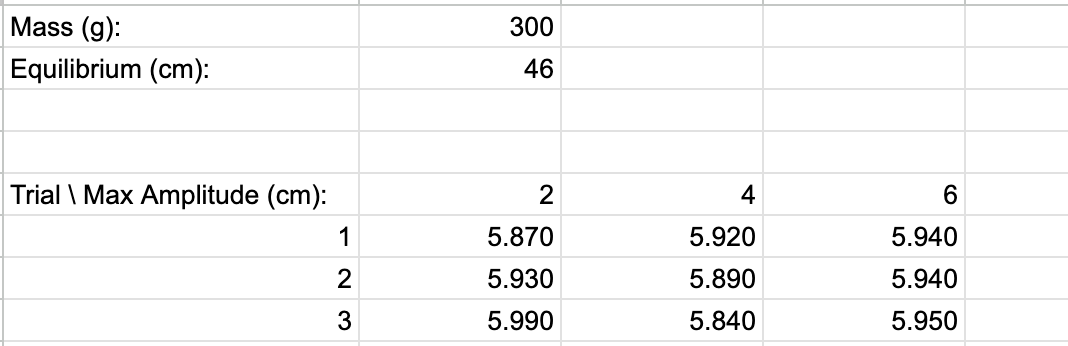
\includegraphics[width=\linewidth]{dynamic_3.png}
        \label{fig:graph_m3}
    \end{subfigure}
\end{figure}

\newpage

\subsection{Dynamic Approach - With Detector}
\begin{figure}[ht!]
    \centering
    %top row
    \begin{subfigure}{1\textwidth}
        \centering
        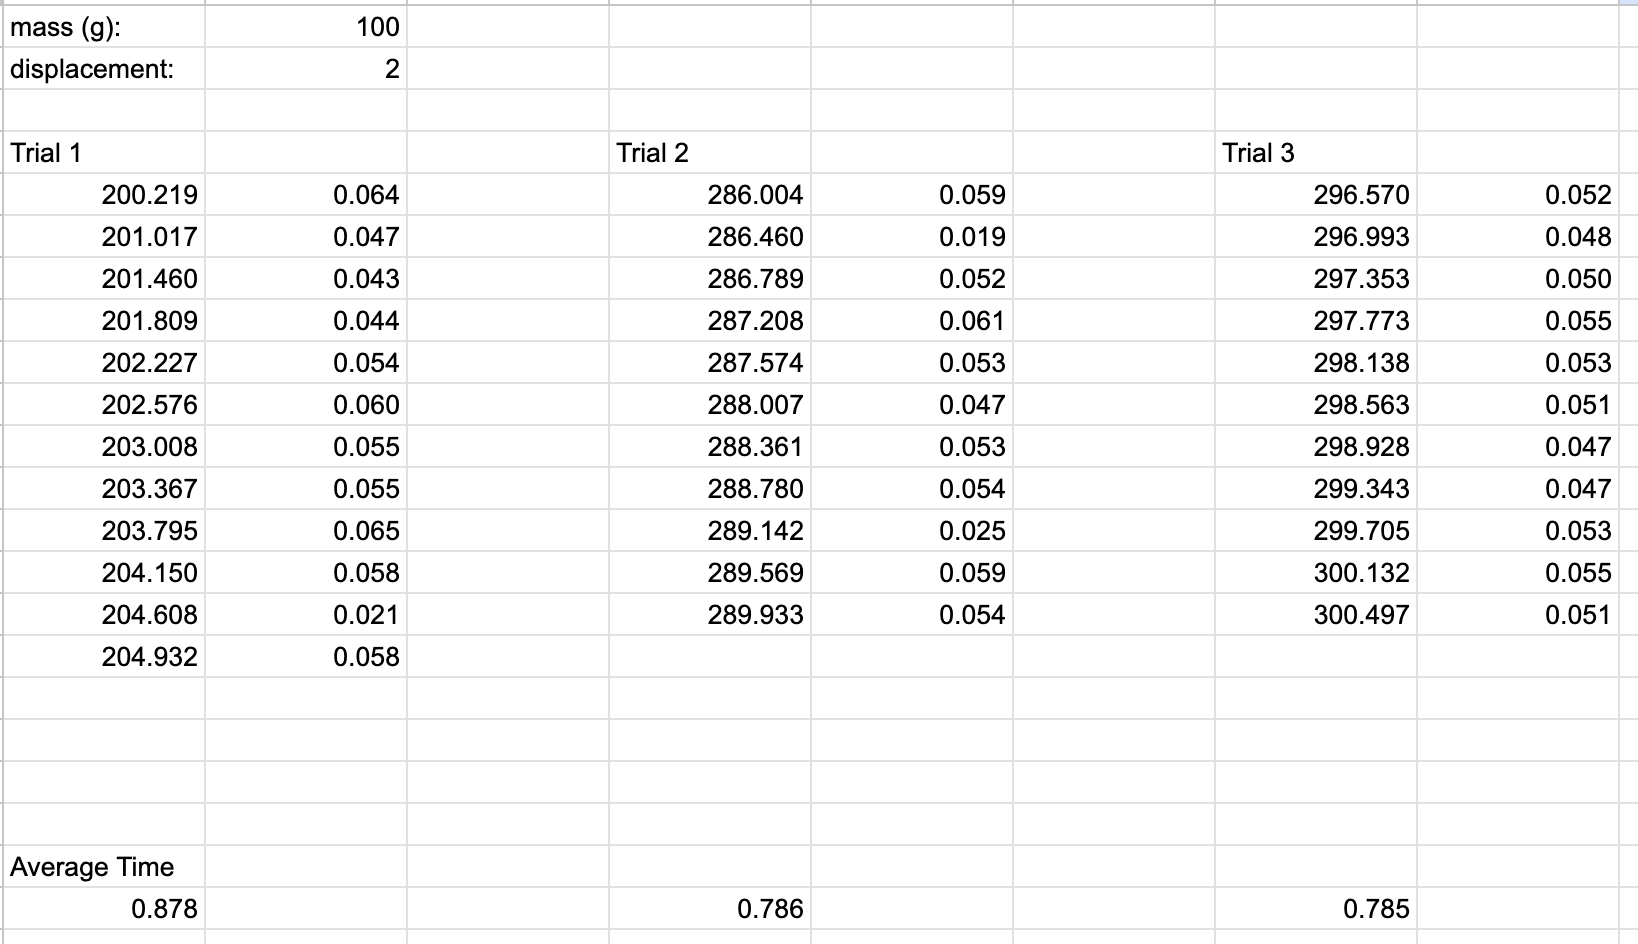
\includegraphics[width=\linewidth]{dynamic_d1.png}
        \label{fig:graph_m1}
    \end{subfigure}
    
    \vspace{1em}

    \begin{subfigure}{1\textwidth}
        \centering
        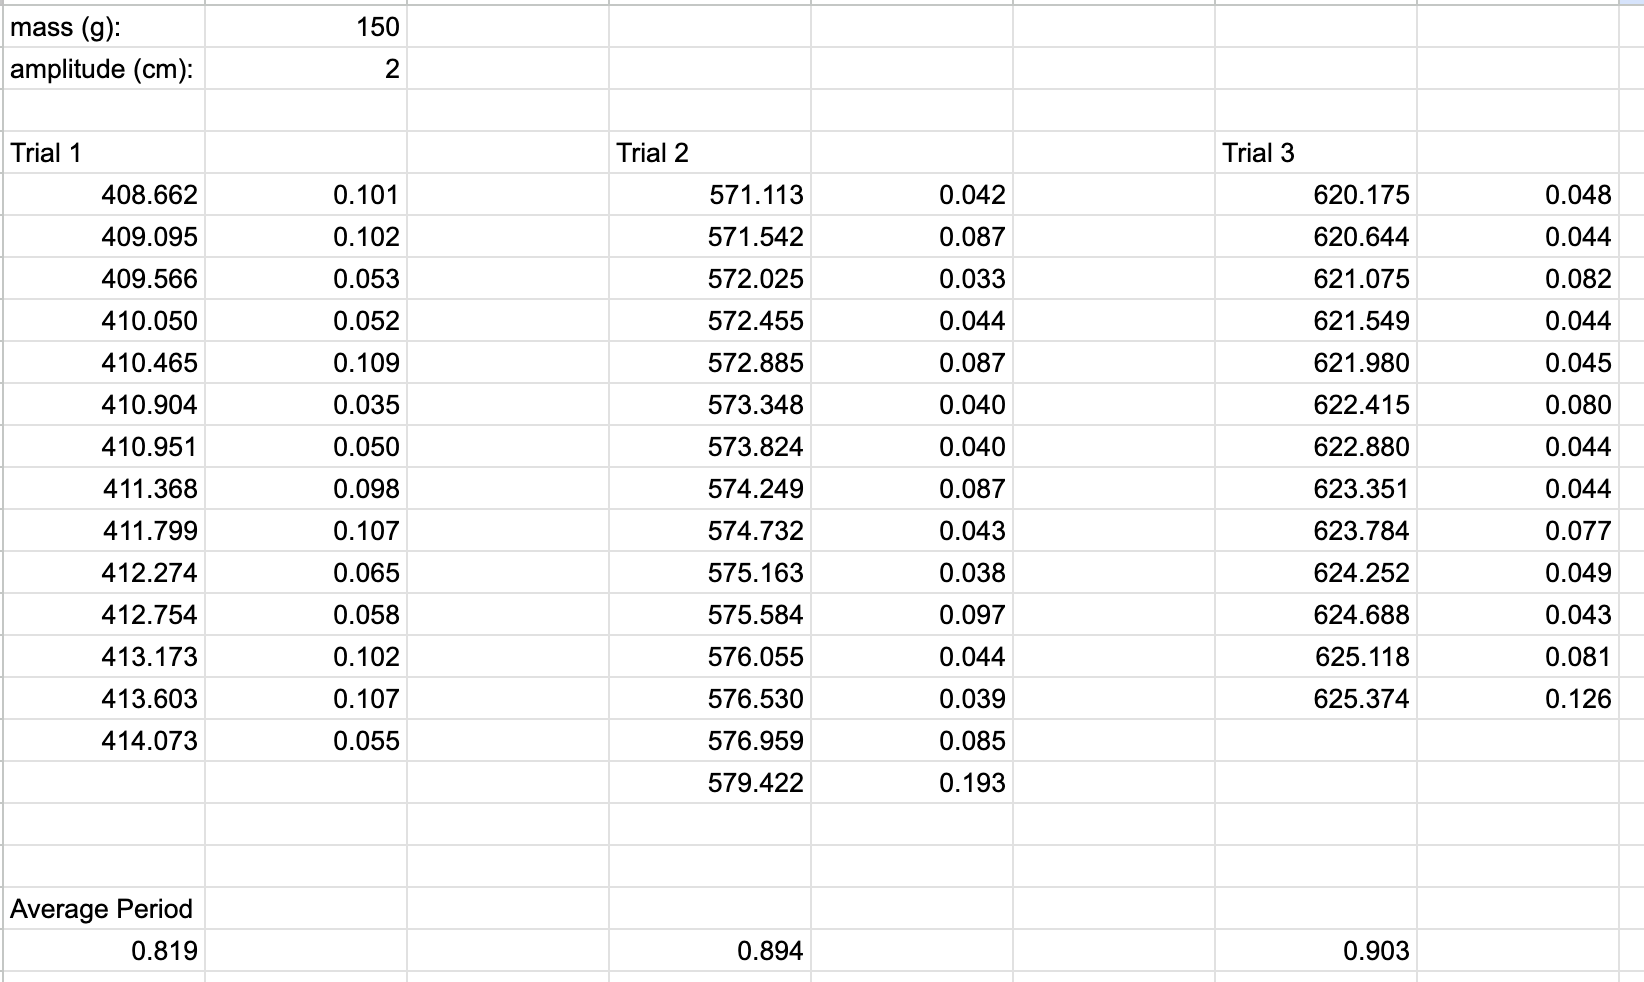
\includegraphics[width=\linewidth]{dynamic_d2.png}
        \label{fig:graph_m2}
    \end{subfigure}
    
    \vspace{1em}

    \begin{subfigure}{1\textwidth}
        \centering
        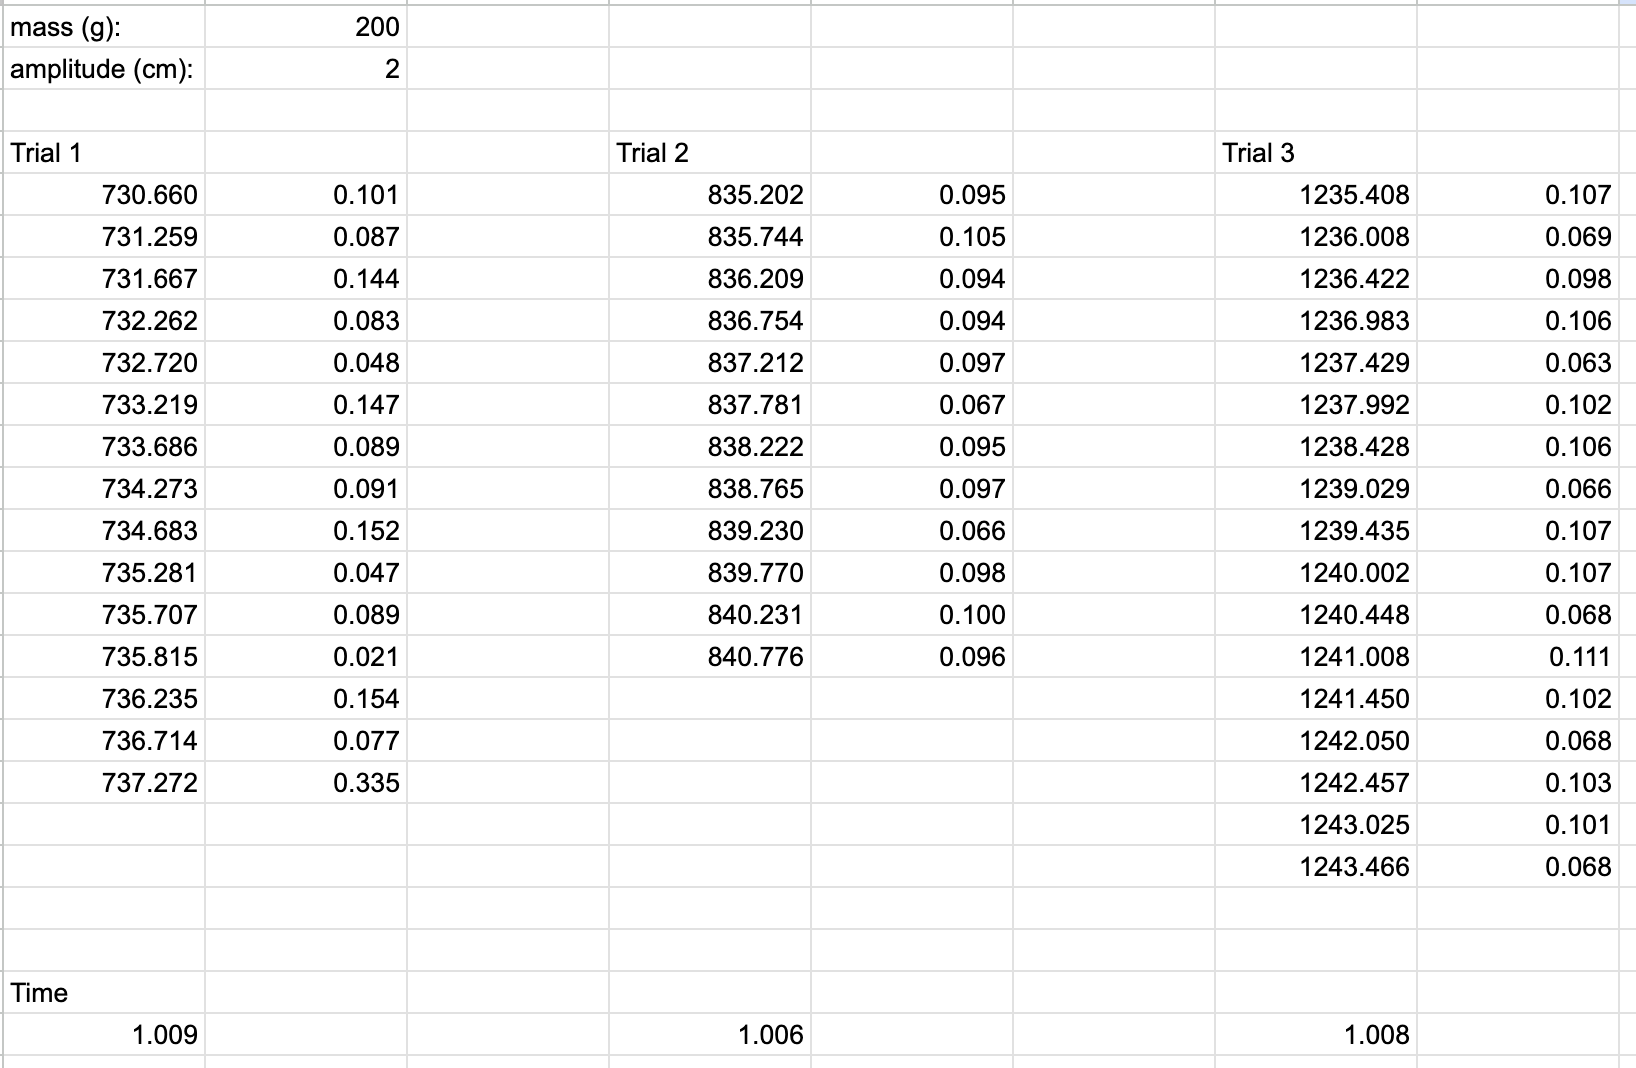
\includegraphics[width=\linewidth]{dynamic_d3.png}
        \label{fig:graph_m3}
    \end{subfigure}
\end{figure}

\end{document}